\sect{LGS}

Eine \textbf{lineare Gleichung in $n$ Variablen} $x_1, \dots, x_n$ hat die Gestalt:
\[a_1 x_1 + \dots + a_n x_n = b\]
wobei $a_1, \dots, a_n$ und $b$ gegebene reelle Konstanten sind.
Die reellen Zahlen $a_i$ mit $i = 1, \dots, n$ nennt man die \textbf{Koeffizienten} der Gleichung und $b \in \R$ ist die \textbf{rechte Seite} der Gleichung.

Ein \textbf{lineares Gleichungssystem} (LGS) besteht aus $m$ linearen Gleichungen mit $n$ Unbekannten $x_1, \dots, x_n$.
Ein solches System hat die folgende Gestalt:
\[
    \setlength\arraycolsep{0pt}
    \left\{
    \begin{array}{*{3}{cC}c}
        a_{11} x_1 & + & \ldots & + & a_{1n} x_n & = & b_1    \\
        \vdots     & + & \vdots & + & \vdots     & = & \vdots \\
        a_{m1} x_1 & + & \ldots & + & a_{mn} x_n & = & b_m
    \end{array}
    \right.
\]

% TODO: Koeffizientenmatrix und Erweiterte Koeffizientenmatrix

\ssect{Elementare Umformungen}

\textbf{Elementare Gleichungsumformungen:}
\begin{itemize}
    \item Vertauschen von den $i$-ten und $j$-ten Gleichungen
    \item Multiplikation der $i$-ten Gleichung mit Skalar $\lambda \neq 0$
    \item Addition eines $\lambda$-fachen der $j$-ten Gleichung zu der $i$-ten Gleichung
\end{itemize}

\textbf{Satz:} Elementare Gleichungsumformungen ändern die Lösungsmenge eines LGS nicht.

\textbf{Elementare Zeilenumformungen:}
\begin{itemize}
    \item Vertauschen von den $i$-ten und $j$-ten Zeilen
    \item Multiplikation der $i$-ten Zeilen mit einem Skalar $\lambda \neq 0$
    \item Addition eines $\lambda$-fachen der $j$-ten Zeile zu der $i$-ten Zeile
\end{itemize}

\ssect{Zeilenstufenform}

Eine Matrix hat \textbf{Zeilenstufenform (ZSF)}, wenn:
\begin{itemize}
    \item Alle Zeilen, die nur Nullen enthalten, stehen in den untersten Zeilen der Matrix.
    \item Wenn eine Zeile nicht nur aus Nullen besteht, so ist die erste von Null verschiedene Zahl eine Eins.
    Sie wird als \textbf{führende Eins} der Zeile bezeichnet.
    \item In zwei aufeinanderfolgenden Zeilen, die nicht verschwindende Elemente besitzen, steht die führende Eins der unteren Zeile rechts von der führenden Eins der oberen Zeile.
\end{itemize}

Eine Matrix in ZSF ist zudem in der \textbf{reduzierten Zeilenstufenform}, falls
\begin{itemize}
    \item eine Spalte, die eine führende Eins enthält, keine weiteren von Null verschiedenen Einträge hat
\end{itemize}

\ssect{Gauss-Jordan-Verfahren}

\begin{enumerate}
    \item Wir bestimmen die am weitesten Links stehende Spalte, die von Null verschiedene Werte enthält.
    \item Ist die oberste Zahl der in Schritt 1 gefundenen Spalte eine Null, dann vertauschen wir die erste Zeile mit einer geeigneten anderen Zeile (1. Zeilenumformung).
    \item Ist $a$ das erste Element der in Schritt 1 gefundene Spalte, dann dividieren wir die erste Zeile durch $a$, um die führende Eins zu erzeugen.
    Man nennt das Element $a$ das Pivotelement (2. Zeilenumformung).
    \item Wir addieren passende Vielfache der ersten Zeile zu den übrigen Zeilen, um unterhalb der führenden Eins Nullen zu erzeugen (3. Zeilenumformung).
    \item Wir wenden die ersten vier Schritte auf den Teil der Matrix an, den wir durch Streichen der ersten Zeile erhalten, und wiederholen dieses Verfahren, bis die erweiterte Koeffizientenmatrix Zeilenstufenform hat.
    \item Mit der letzten nicht verschwindenden Zeile beginnend, addieren wir geeignete Vielfache jeder Zeile zu den darüber liegenden Zeilen, um über den führenden Einsen Nullen zu
    erzeugen (3. Zeilenumformung).
\end{enumerate}

\ssect{Gauss-Verfahren}

\begin{enumerate}
    \item Wir führen die Schritte 1.\ bis 5.\ wie beim Gauss-Jordan-Verfahren durch.
    \item Wir lösen das System in ZSF durch Rückwärtseinsetzen.
\end{enumerate}

\ssect{Lösungsmenge von LGS}

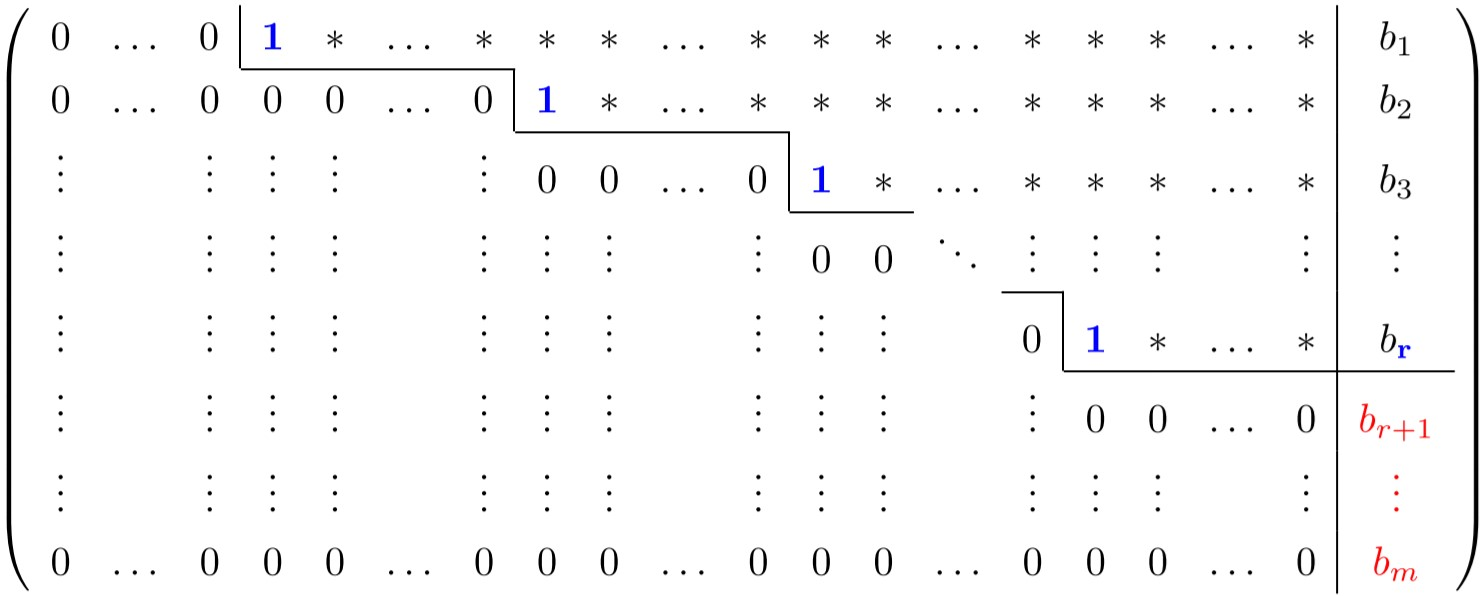
\includegraphics[scale=0.233]{zeilenstufenform}

Sei $r$ die Anzahl der Nicht-Nullzeilen in der ZSF der Koeffizientenmatrix $A$.
Dann heisst $r$ der Rang der Matrix $A$.

\textbf{Anmerkung:}
\begin{itemize}
    \item Es gilt: $r \geq 0$ und $r \leq m$
    \item Die Anzahl der führenden Variablen ist gleich $r$.
    Somit muss auch $r \leq n$ gelten.
    \item Es gibt $n - r$ freie Variablen.
\end{itemize}

Seien $A \vec{x} = \vec{b}$ ein LGS mit $m$ Gleichungen und $n$ Unbekannten, und $r = rg(A)$.\\
Das LGS ist nur \textbf{lösbar}, wenn: $r = rg(A \mid \vec{b})$\\
D.h.\ wenn entweder $r < m$ und $b_k = 0$, $k = r + 1, \dots, m$ oder $r = m$.

Im Falle der Lösbarkeit besitzt das LGS:
\begin{itemize}
    \item Für $r = n$: \textbf{Genau eine Lösung}
    \item Für $r < n$: \textbf{Unendlich viele Lösungen}, wobei die Anzahl der freien Variablen gleich $n - r$ ist.
\end{itemize}

\columnbreak

% TODO: Berechnung der Inverse Matrix